% Generated by scripts/build_rq3_report.py — do not edit by hand.
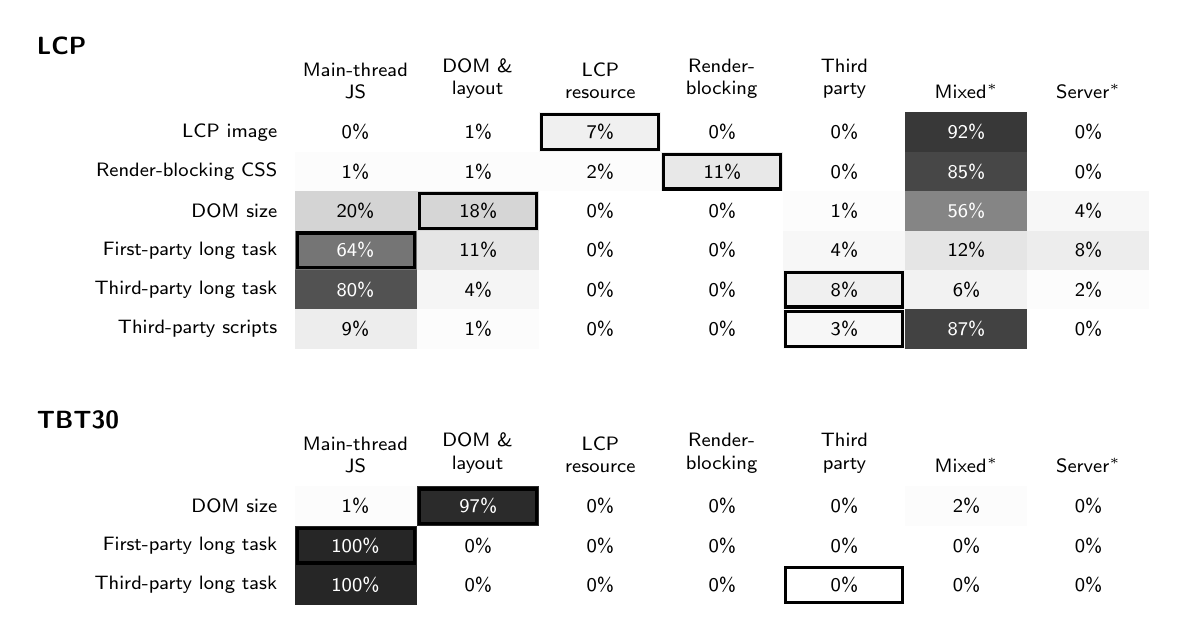
\begin{tikzpicture}[font=\sffamily\scriptsize]
\node[font=\sffamily\bfseries\small, anchor=west] at (0,0.00) {LCP};
\node[align=center, anchor=south] at (4.17,-0.80) {Main-thread\\JS};
\node[align=center, anchor=south] at (5.72,-0.80) {DOM \&\\layout};
\node[align=center, anchor=south] at (7.28,-0.80) {LCP\\resource};
\node[align=center, anchor=south] at (8.82,-0.80) {Render-\\blocking};
\node[align=center, anchor=south] at (10.38,-0.80) {Third\\party};
\node[align=center, anchor=south] at (11.93,-0.80) {Mixed$^{*}$};
\node[align=center, anchor=south] at (13.48,-0.80) {Server$^{*}$};
\node[anchor=east] at (3.30,-1.10) {LCP image};
\fill[black!0] (3.40,-1.35) rectangle (4.95,-0.85);
\node[black] at (4.17,-1.10) {0\%};
\fill[black!0] (4.95,-1.35) rectangle (6.50,-0.85);
\node[black] at (5.73,-1.10) {1\%};
\fill[black!6] (6.50,-1.35) rectangle (8.05,-0.85);
\node[black] at (7.28,-1.10) {7\%};
\draw[very thick] (6.53,-1.32) rectangle (8.02,-0.88);
\fill[black!0] (8.05,-1.35) rectangle (9.60,-0.85);
\node[black] at (8.83,-1.10) {0\%};
\fill[black!0] (9.60,-1.35) rectangle (11.15,-0.85);
\node[black] at (10.38,-1.10) {0\%};
\fill[black!78] (11.15,-1.35) rectangle (12.70,-0.85);
\node[white] at (11.93,-1.10) {92\%};
\fill[black!0] (12.70,-1.35) rectangle (14.25,-0.85);
\node[black] at (13.48,-1.10) {0\%};
\node[anchor=east] at (3.30,-1.60) {Render-blocking CSS};
\fill[black!1] (3.40,-1.85) rectangle (4.95,-1.35);
\node[black] at (4.17,-1.60) {1\%};
\fill[black!1] (4.95,-1.85) rectangle (6.50,-1.35);
\node[black] at (5.73,-1.60) {1\%};
\fill[black!1] (6.50,-1.85) rectangle (8.05,-1.35);
\node[black] at (7.28,-1.60) {2\%};
\fill[black!9] (8.05,-1.85) rectangle (9.60,-1.35);
\node[black] at (8.83,-1.60) {11\%};
\draw[very thick] (8.08,-1.82) rectangle (9.57,-1.38);
\fill[black!0] (9.60,-1.85) rectangle (11.15,-1.35);
\node[black] at (10.38,-1.60) {0\%};
\fill[black!72] (11.15,-1.85) rectangle (12.70,-1.35);
\node[white] at (11.93,-1.60) {85\%};
\fill[black!0] (12.70,-1.85) rectangle (14.25,-1.35);
\node[black] at (13.48,-1.60) {0\%};
\node[anchor=east] at (3.30,-2.10) {DOM size};
\fill[black!17] (3.40,-2.35) rectangle (4.95,-1.85);
\node[black] at (4.17,-2.10) {20\%};
\fill[black!16] (4.95,-2.35) rectangle (6.50,-1.85);
\node[black] at (5.73,-2.10) {18\%};
\draw[very thick] (4.98,-2.32) rectangle (6.47,-1.88);
\fill[black!0] (6.50,-2.35) rectangle (8.05,-1.85);
\node[black] at (7.28,-2.10) {0\%};
\fill[black!0] (8.05,-2.35) rectangle (9.60,-1.85);
\node[black] at (8.83,-2.10) {0\%};
\fill[black!1] (9.60,-2.35) rectangle (11.15,-1.85);
\node[black] at (10.38,-2.10) {1\%};
\fill[black!48] (11.15,-2.35) rectangle (12.70,-1.85);
\node[white] at (11.93,-2.10) {56\%};
\fill[black!3] (12.70,-2.35) rectangle (14.25,-1.85);
\node[black] at (13.48,-2.10) {4\%};
\node[anchor=east] at (3.30,-2.60) {First-party long task};
\fill[black!54] (3.40,-2.85) rectangle (4.95,-2.35);
\node[white] at (4.17,-2.60) {64\%};
\draw[very thick] (3.43,-2.82) rectangle (4.92,-2.38);
\fill[black!10] (4.95,-2.85) rectangle (6.50,-2.35);
\node[black] at (5.73,-2.60) {11\%};
\fill[black!0] (6.50,-2.85) rectangle (8.05,-2.35);
\node[black] at (7.28,-2.60) {0\%};
\fill[black!0] (8.05,-2.85) rectangle (9.60,-2.35);
\node[black] at (8.83,-2.60) {0\%};
\fill[black!3] (9.60,-2.85) rectangle (11.15,-2.35);
\node[black] at (10.38,-2.60) {4\%};
\fill[black!10] (11.15,-2.85) rectangle (12.70,-2.35);
\node[black] at (11.93,-2.60) {12\%};
\fill[black!7] (12.70,-2.85) rectangle (14.25,-2.35);
\node[black] at (13.48,-2.60) {8\%};
\node[anchor=east] at (3.30,-3.10) {Third-party long task};
\fill[black!68] (3.40,-3.35) rectangle (4.95,-2.85);
\node[white] at (4.17,-3.10) {80\%};
\fill[black!4] (4.95,-3.35) rectangle (6.50,-2.85);
\node[black] at (5.73,-3.10) {4\%};
\fill[black!0] (6.50,-3.35) rectangle (8.05,-2.85);
\node[black] at (7.28,-3.10) {0\%};
\fill[black!0] (8.05,-3.35) rectangle (9.60,-2.85);
\node[black] at (8.83,-3.10) {0\%};
\fill[black!6] (9.60,-3.35) rectangle (11.15,-2.85);
\node[black] at (10.38,-3.10) {8\%};
\draw[very thick] (9.63,-3.32) rectangle (11.12,-2.88);
\fill[black!5] (11.15,-3.35) rectangle (12.70,-2.85);
\node[black] at (11.93,-3.10) {6\%};
\fill[black!1] (12.70,-3.35) rectangle (14.25,-2.85);
\node[black] at (13.48,-3.10) {2\%};
\node[anchor=east] at (3.30,-3.60) {Third-party scripts};
\fill[black!7] (3.40,-3.85) rectangle (4.95,-3.35);
\node[black] at (4.17,-3.60) {9\%};
\fill[black!1] (4.95,-3.85) rectangle (6.50,-3.35);
\node[black] at (5.73,-3.60) {1\%};
\fill[black!0] (6.50,-3.85) rectangle (8.05,-3.35);
\node[black] at (7.28,-3.60) {0\%};
\fill[black!0] (8.05,-3.85) rectangle (9.60,-3.35);
\node[black] at (8.83,-3.60) {0\%};
\fill[black!3] (9.60,-3.85) rectangle (11.15,-3.35);
\node[black] at (10.38,-3.60) {3\%};
\draw[very thick] (9.63,-3.82) rectangle (11.12,-3.38);
\fill[black!74] (11.15,-3.85) rectangle (12.70,-3.35);
\node[white] at (11.93,-3.60) {87\%};
\fill[black!0] (12.70,-3.85) rectangle (14.25,-3.35);
\node[black] at (13.48,-3.60) {0\%};
\node[font=\sffamily\bfseries\small, anchor=west] at (0,-4.75) {TBT30};
\node[align=center, anchor=south] at (4.17,-5.55) {Main-thread\\JS};
\node[align=center, anchor=south] at (5.72,-5.55) {DOM \&\\layout};
\node[align=center, anchor=south] at (7.28,-5.55) {LCP\\resource};
\node[align=center, anchor=south] at (8.82,-5.55) {Render-\\blocking};
\node[align=center, anchor=south] at (10.38,-5.55) {Third\\party};
\node[align=center, anchor=south] at (11.93,-5.55) {Mixed$^{*}$};
\node[align=center, anchor=south] at (13.48,-5.55) {Server$^{*}$};
\node[anchor=east] at (3.30,-5.85) {DOM size};
\fill[black!1] (3.40,-6.10) rectangle (4.95,-5.60);
\node[black] at (4.17,-5.85) {1\%};
\fill[black!83] (4.95,-6.10) rectangle (6.50,-5.60);
\node[white] at (5.73,-5.85) {97\%};
\draw[very thick] (4.98,-6.07) rectangle (6.47,-5.63);
\fill[black!0] (6.50,-6.10) rectangle (8.05,-5.60);
\node[black] at (7.28,-5.85) {0\%};
\fill[black!0] (8.05,-6.10) rectangle (9.60,-5.60);
\node[black] at (8.83,-5.85) {0\%};
\fill[black!0] (9.60,-6.10) rectangle (11.15,-5.60);
\node[black] at (10.38,-5.85) {0\%};
\fill[black!1] (11.15,-6.10) rectangle (12.70,-5.60);
\node[black] at (11.93,-5.85) {2\%};
\fill[black!0] (12.70,-6.10) rectangle (14.25,-5.60);
\node[black] at (13.48,-5.85) {0\%};
\node[anchor=east] at (3.30,-6.35) {First-party long task};
\fill[black!85] (3.40,-6.60) rectangle (4.95,-6.10);
\node[white] at (4.17,-6.35) {100\%};
\draw[very thick] (3.43,-6.57) rectangle (4.92,-6.13);
\fill[black!0] (4.95,-6.60) rectangle (6.50,-6.10);
\node[black] at (5.73,-6.35) {0\%};
\fill[black!0] (6.50,-6.60) rectangle (8.05,-6.10);
\node[black] at (7.28,-6.35) {0\%};
\fill[black!0] (8.05,-6.60) rectangle (9.60,-6.10);
\node[black] at (8.83,-6.35) {0\%};
\fill[black!0] (9.60,-6.60) rectangle (11.15,-6.10);
\node[black] at (10.38,-6.35) {0\%};
\fill[black!0] (11.15,-6.60) rectangle (12.70,-6.10);
\node[black] at (11.93,-6.35) {0\%};
\fill[black!0] (12.70,-6.60) rectangle (14.25,-6.10);
\node[black] at (13.48,-6.35) {0\%};
\node[anchor=east] at (3.30,-6.85) {Third-party long task};
\fill[black!85] (3.40,-7.10) rectangle (4.95,-6.60);
\node[white] at (4.17,-6.85) {100\%};
\fill[black!0] (4.95,-7.10) rectangle (6.50,-6.60);
\node[black] at (5.73,-6.85) {0\%};
\fill[black!0] (6.50,-7.10) rectangle (8.05,-6.60);
\node[black] at (7.28,-6.85) {0\%};
\fill[black!0] (8.05,-7.10) rectangle (9.60,-6.60);
\node[black] at (8.83,-6.85) {0\%};
\fill[black!0] (9.60,-7.10) rectangle (11.15,-6.60);
\node[black] at (10.38,-6.85) {0\%};
\draw[very thick] (9.63,-7.07) rectangle (11.12,-6.63);
\fill[black!0] (11.15,-7.10) rectangle (12.70,-6.60);
\node[black] at (11.93,-6.85) {0\%};
\fill[black!0] (12.70,-7.10) rectangle (14.25,-6.60);
\node[black] at (13.48,-6.85) {0\%};
\end{tikzpicture}
